%======================================================================
% University of Stuttgart Template for LaTeX 
% Last Updated April, 2021 
% by Beatriz Negreiros

% DISCLAIMER
% To the best of the Author's knowledge, this template satisfies the current University of Stuttgart thesis requirements.
% However, it is your responsibility to assure that you have met all requirements of the University and your particular department.
% Also note that there are explanatory comments and tips throughout this template.
%======================================================================

\documentclass[12pt,twoside]{report}

%-----------------PREAMBLE------------------------------
% Document Formatting
\usepackage[english]{babel}
\usepackage{microtype}
\usepackage{parskip}
\usepackage{fourier}
\usepackage{fancyhdr}

% Preamble for references 
%\usepackage{fancyref}
\usepackage{hyperref}
\usepackage{apacite}

% Formatting Preamble
\usepackage[top=1.5in, bottom=1in, left=1in, right=1in]{geometry}

% Graphics Preamble
\usepackage{graphicx}
\graphicspath{ {./images/} }
\usepackage[font={small}, hang]{caption}

% Mathematics Preamble
\usepackage{amsmath}
\newcommand{\R}{\mathbb{R}}

% Other
\usepackage{gensymb}  %inserts degree 
\usepackage[inline, shortlabels]{enumitem} % letter type of listing (a)..(b)..

% Document
%\title{\textbf{Fuzzy-Kappa map comparison to assess the performance of hydro-morphodynamic models}}
\title{\textbf{[Name of the Thesis]}}
\author{[Student name]}

% Macros - here you can define macros for shortening the writing of large words, for instance:
\def\rmse{Root Mean Squared Error}


% Begin of document
%======================================================================
\begin{document}

\begin{titlepage}
	\begin{large}
	\begin{center}
	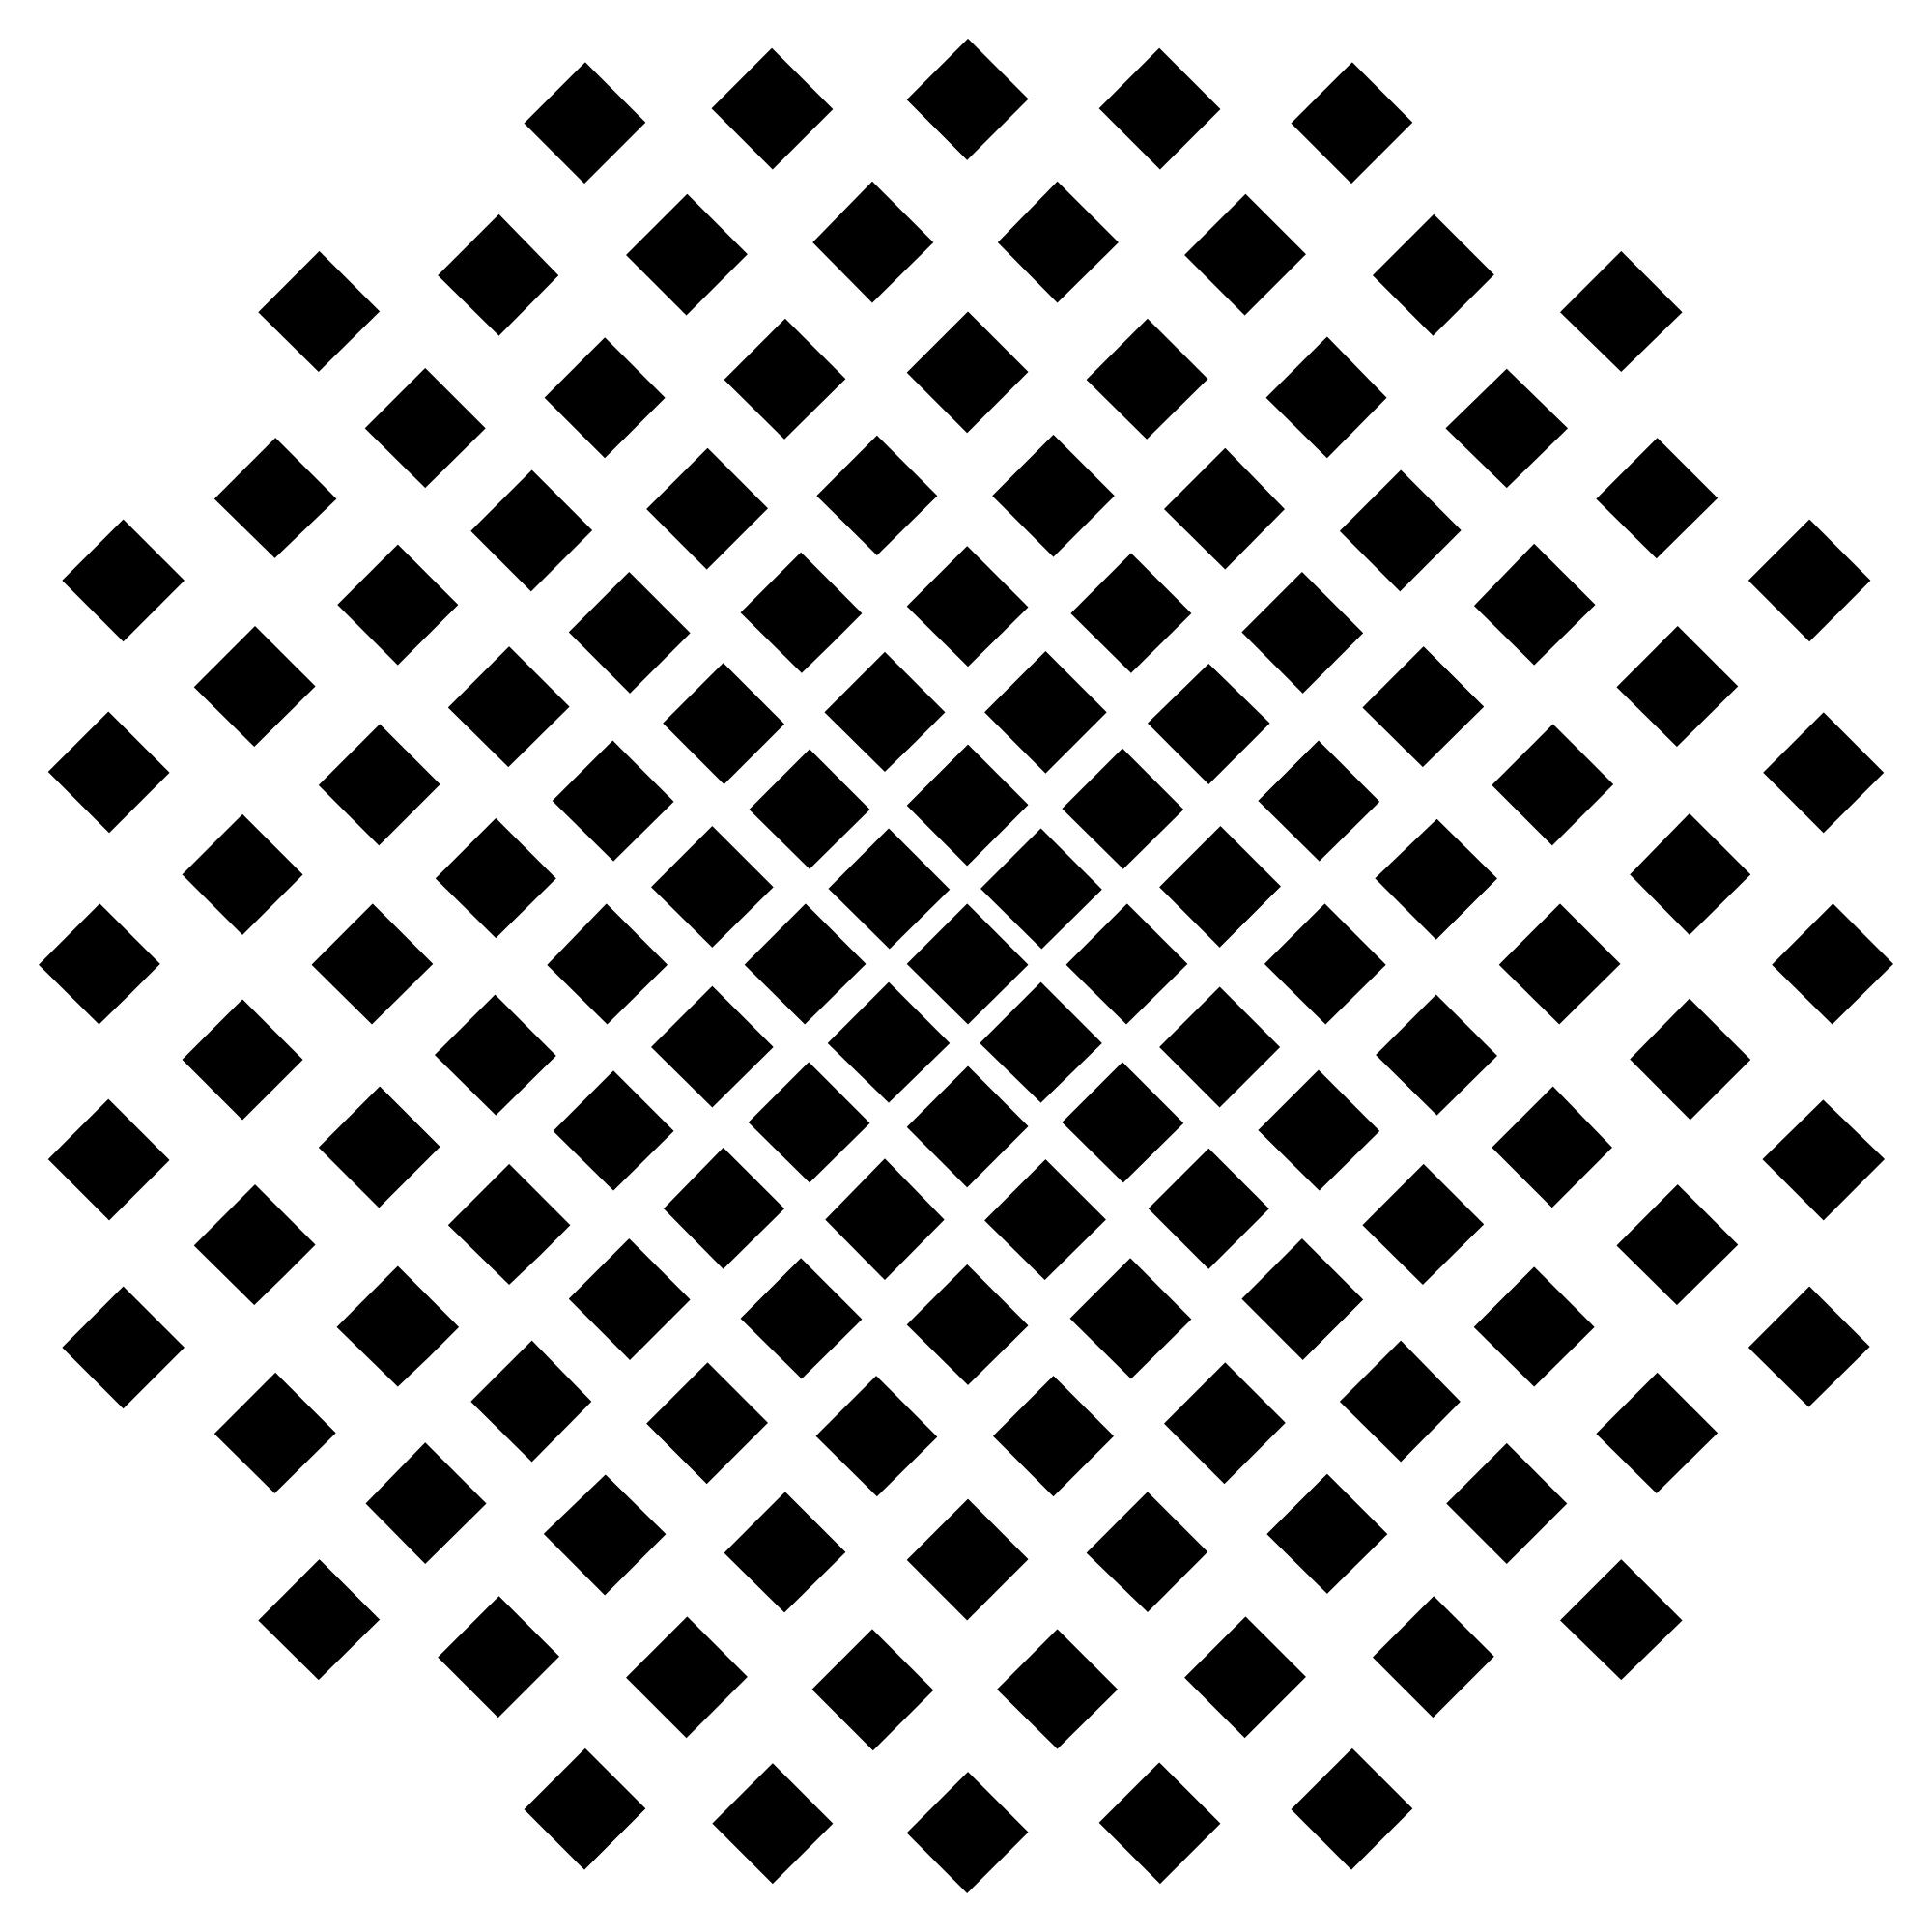
\includegraphics[width=2cm]{uni_logo.png}
	\hspace*{4in}
	
\includegraphics[width=3.5cm]{Logo_LWW.png}\\
		Universit{\"a}t Stuttgart\\
		\vspace{1cm}
		[Name of the department]\\
		
		[Name of the institute]\\
		
		\vspace{1.0cm}
		\begin{Huge}
			\textbf{[Thesis name]}\\
		\end{Huge}
		\vspace{1.5cm}
		Master's Thesis % It's not Master Thesis, nor master thesis, but exactly how it's written here
		
		\vspace{1.5cm}
		Student's name\\
		(Course's name)
		\vspace{1.5cm}
		
		[Matriculation Number] \\
		
		\date{\today}
	\end{center}
		\vspace{1.5cm}
		\begin{tabular}{rl}
			\textbf{Examiner:} & [Name of examiner] \\
			\textbf{Supervisors:} & [Supervisor 1] \\ & [Supervisor 2]
		\end{tabular}
	
	\end{large}
\end{titlepage}
		

\clearpage

\pagenumbering{roman}


\chapter*{Acknowledgements}
{

}
\addcontentsline{toc}{chapter}{Acknowledgements}

\chapter*{Abstract}
{

}
\addcontentsline{toc}{chapter}{Abstract}

% List of contents, figures and tables
\tableofcontents
\clearpage

\listoffigures
\addcontentsline{toc}{chapter}{List of Figures}

\listoftables
\addcontentsline{toc}{chapter}{List of Tables}

% Beginning of chapters
\pagestyle{fancy}
\fancyhf{}
\fancyhead[LE,RO]{\nouppercase{\leftmark}}
\fancyhead[RE,LO]{\nouppercase{\rightmark}}
\fancyfoot[LE,RO]{\thepage}
\renewcommand{\headrulewidth}{1.0pt}

\chapter{Introduction}
\label{ch:introduction}
\pagenumbering{arabic}
\setcounter{page}{1}




	\section{Background}
	\label{subsec:background}
	write here

	\section{Something Location}
	\label{subsec:somelocation}

	write here

	See more in ~\autoref{subsec:background}
	write here
	
	\begin{center}
	\end{center}
	
\chapter{State-of-the-art}
\label{ch:stateart}

\section{Previous works}
\label{sec:prevworks}
	
	% For referring to sections or chapter you rpesented before:
	As explained in section~\ref{sec:notlogic}
	
	
\section{Types of Something}
\label{sec:typesome}

		
		\subsection{somethingsomething}
		\label{subsec:somesome}
		
		As the Table~\ref{tb:typesomething} shows.
		
		\subsection{somethingnothing}
		\label{subsec:somenoth}
		
        \begin{table}[]
            \centering
            \begin{tabular}{ll}
            \hline
            \textbf{Thing} & \textbf{Utilization} \\
            \hline
                something & something \\
                something & something \\
                something & something \\
                \hline
            \end{tabular}
            \caption{Types of something}
            \label{tb:typesomething}
        \end{table}
		
\section{Something Statistics}
\label{sec:somestatistics}
	
		As shown in Equation~\ref{eq:happiness}
		\begin{equation}\label{eq:happiness}
			happiness=\frac{EmptyCup+coffee}{EmptyCups}
		\end{equation}	
	
	
\section{Nothing Logic}
\label{sec:notlogic}
	
		\subsection{The logic underlying something}
		\label{subsec:logicunderlying}
    	
    	
    	
		\subsection{Concepts and terminology}
		\label{subsec:conceptsterm}	
		
    	\subsubsection*{Something set rules}

    	Understanding the semantics of something

\section{Something or nothing?}
\label{sec:someornot}

	\subsubsection{Some non-sense?}
	
    	
    	
    \subsubsection{Write happily!}
    	
    	
    	
    

\chapter{Methods}
\label{ch:methods}	

\chapter{Results}
\label{ch:results}

\chapter{Discussion}
\label{ch:discussion}

\chapter{Conclusions}
\label{ch:conclusion}
{
More information is provided by other sources \cite{mittelbach2004latex, goossens1994latex}.
}


\pagestyle{fancy}
\fancyhf{}
\fancyhead[LE,RO]{\nouppercase{\rightmark}}
\fancyfoot[LE,RO]{\thepage}
\renewcommand{\headrulewidth}{1.0pt}

\bibliographystyle{apacite}
\bibliography{References}


% The \appendix statement indicates the beginning of the appendices.
\appendix
% Add an un-numbered title page before the appendices and a line in the Table of Contents
\chapter*{Appendices}
\addcontentsline{toc}{chapter}{Appendices}
% Appendices are just more chapters, with different labeling (letters instead of numbers).
\chapter[Appendix]{Something to complement other things}
\label{AppendixA}
% Tip 4: Example (above) of how to get a shorter chapter title for the Table of Contents 
%======================================================================

\section{[Maps of something]}


\chapter[Appendix]{Something to complement other things}
\label{AppendixA}
% Tip 4: Example (above) of how to get a shorter chapter title for the Table of Contents 
%======================================================================

\section{[Maps of something]}


\end{document}
